\HeadingLevelB{SGX Software Attestation}
\label{sec:sgx_attestation}

The software attestation scheme implemented by SGX follows the principles
outlined in \S~\ref{sec:generic_software_attestation}. An SGX-enabled processor
computes a measurement of the code and data that is loaded in each enclave,
which is similar to the measurement computed by the
TPM~(\S~\ref{sec:sgx_related_tpm}). The software inside an enclave can start a
process that results in an SGX attestation signature, which includes the
enclave's measurement and an enclave message.

\begin{figure}[hbt]
  \centering
  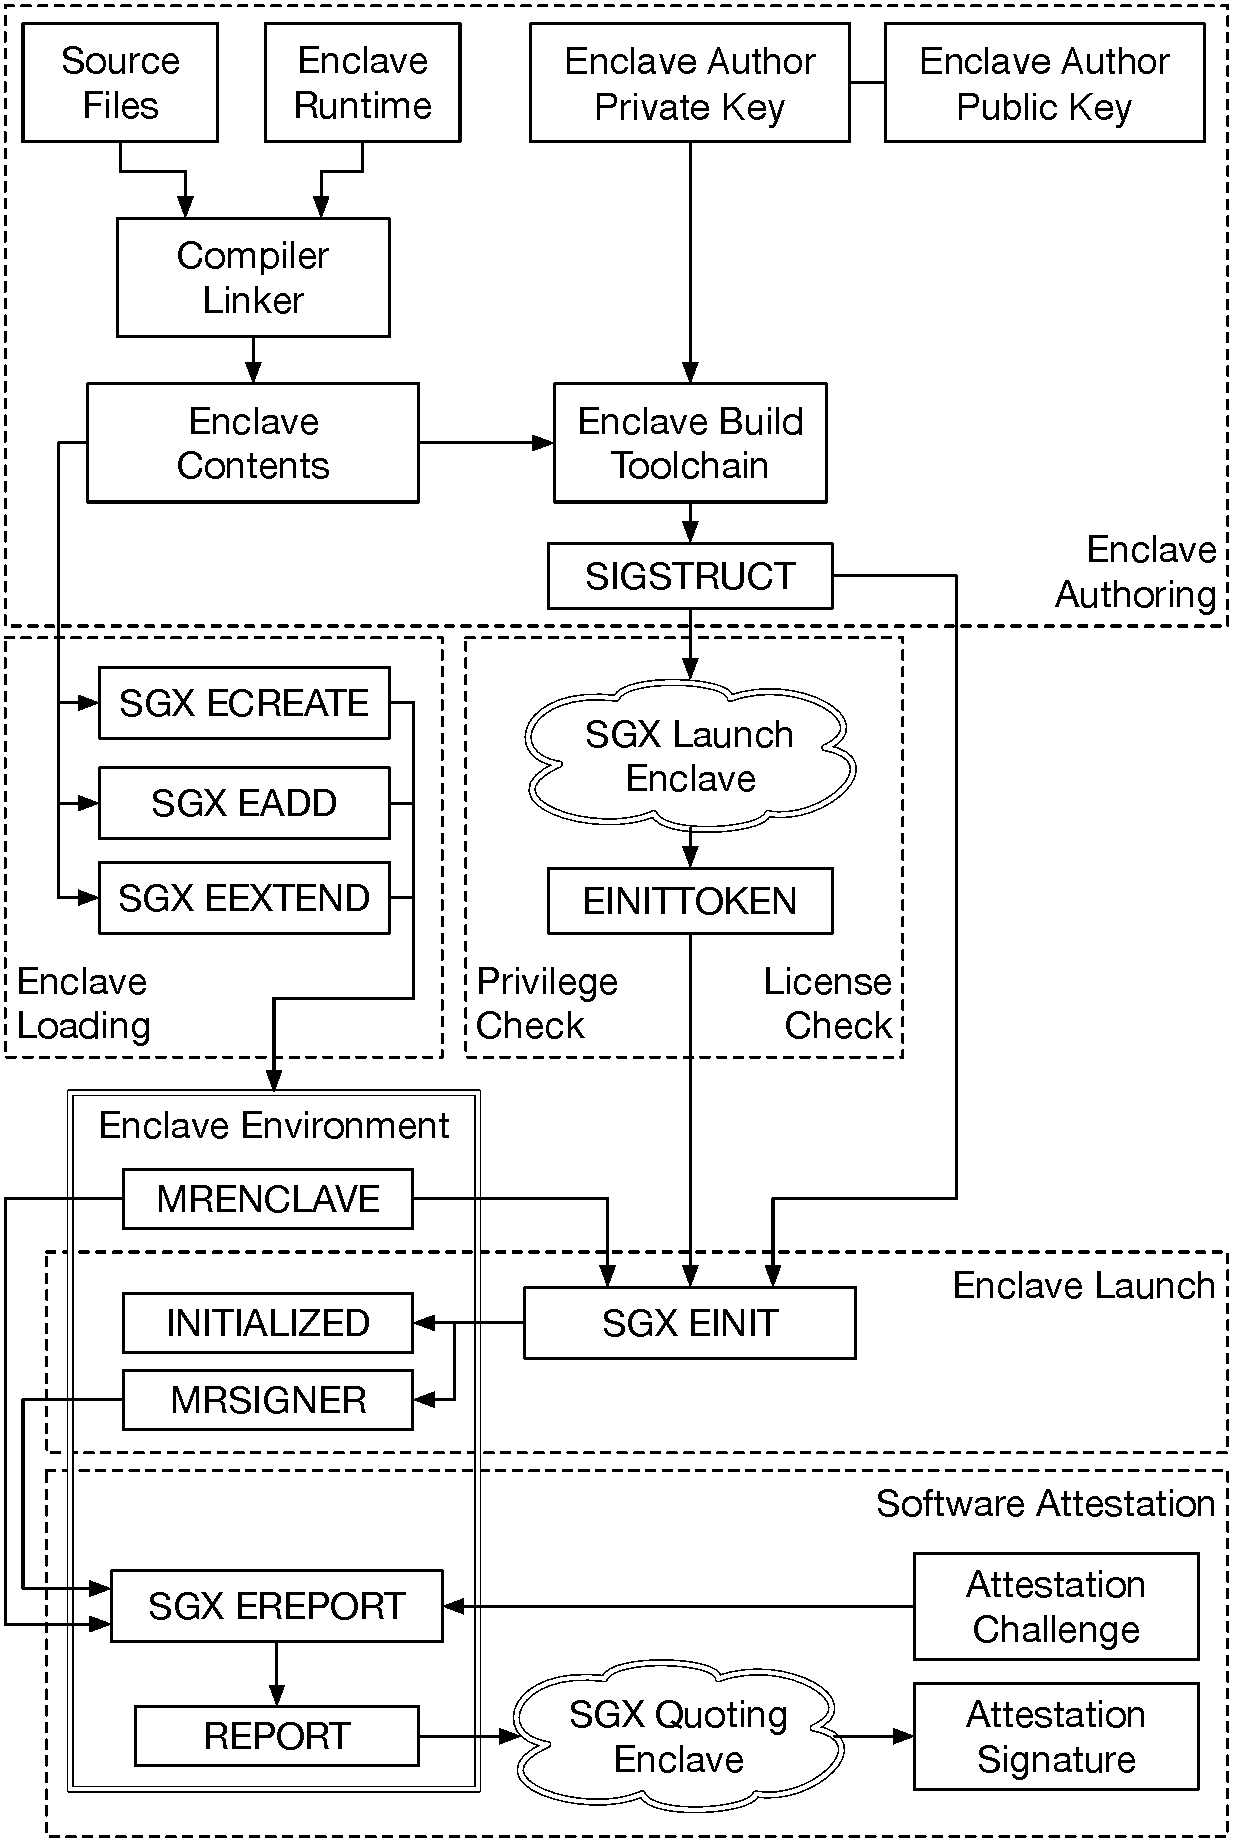
\includegraphics[width=85mm]{figures/sgx_attestation_overview.pdf}
  \caption{
    Setting up an SGX enclave and undergoing the software attestation process
    involves the SGX instructions \texttt{EINIT} and \texttt{EREPORT}, and two
    special enclaves authored by Intel, the SGX Launch Enclave and the SGX
    Quoting Enclave.
  }
  \label{fig:sgx_attestation_overview}
\end{figure}

% EPID signing takes too long for microcode.
%   US 8,972,746 B2 - 21:8-16, 33:16-29, 33:58

The cryptographic primitive used in SGX's attestation signature is too complex
to be implemented in hardware, so the signing process is performed by a
privileged \textit{Quoting Enclave}, which is issued by Intel, and can access
the SGX attestation key. This enclave is discussed in
\S~\ref{sec:sgx_quoting_enclave}.

Pushing the signing functionality into the Quoting Enclave creates the need for
a secure communication path between an enclave undergoing software attestation
and the Quoting Enclave. The SGX design solves this problem with a local
attestation mechanism that can be used by an enclave to prove its identity to
any other enclave hosted by the same SGX-enabled CPU. This scheme, described in
\S~\ref{sec:sgx_ereport}, is implemented by the \texttt{EREPORT} instruction.

% Keys: SDM S 39.4.3
% ISCA SGX Slides 104, 105, 106

The SGX attestation key used by the Quoting Enclave does not exist at the time
SGX-enabled processors leave the factory. The attestation key is provisioned
later, using a process that involves a Provisioning Enclave issued by Intel,
and two special \texttt{EGETKEY}~(~\S~\ref{sec:sgx_egetkey}) key types. The
publicly available details of this process are summarized in
\S~\ref{sec:sgx_quoting_enclave}.

The SGX Launch Enclave and EINITTOKEN structure will be discussed in
\S~\ref{sec:sgx_launch_control}.

\HeadingLevelC{Local Attestation}
\label{sec:sgx_ereport}

% Using REPORTs for Local Attestation: SDM S 39.4.3.2
% EREPORT: SDM S 41.4.1

An enclave proves its identity to another \textit{target enclave} via the
\texttt{EREPORT} instruction shown in Figure~\ref{fig:sgx_ereport}. The SGX
instruction produces an attestation \textit{Report} (REPORT) that
cryptographically binds a message supplied by the enclave with the enclave's
measurement-based~(\S~\ref{sec:sgx_measurement}) and
certificate-based~(\S~\ref{sec:sgx_certificate_identity}) identities. The
cryptographic binding is accomplished by a MAC
tag~(\S~\ref{sec:integrity_crypto}) computed using a symmetric key that is only
shared between the target enclave and the SGX implementation.

\begin{figure}[hbt]
  \centering
  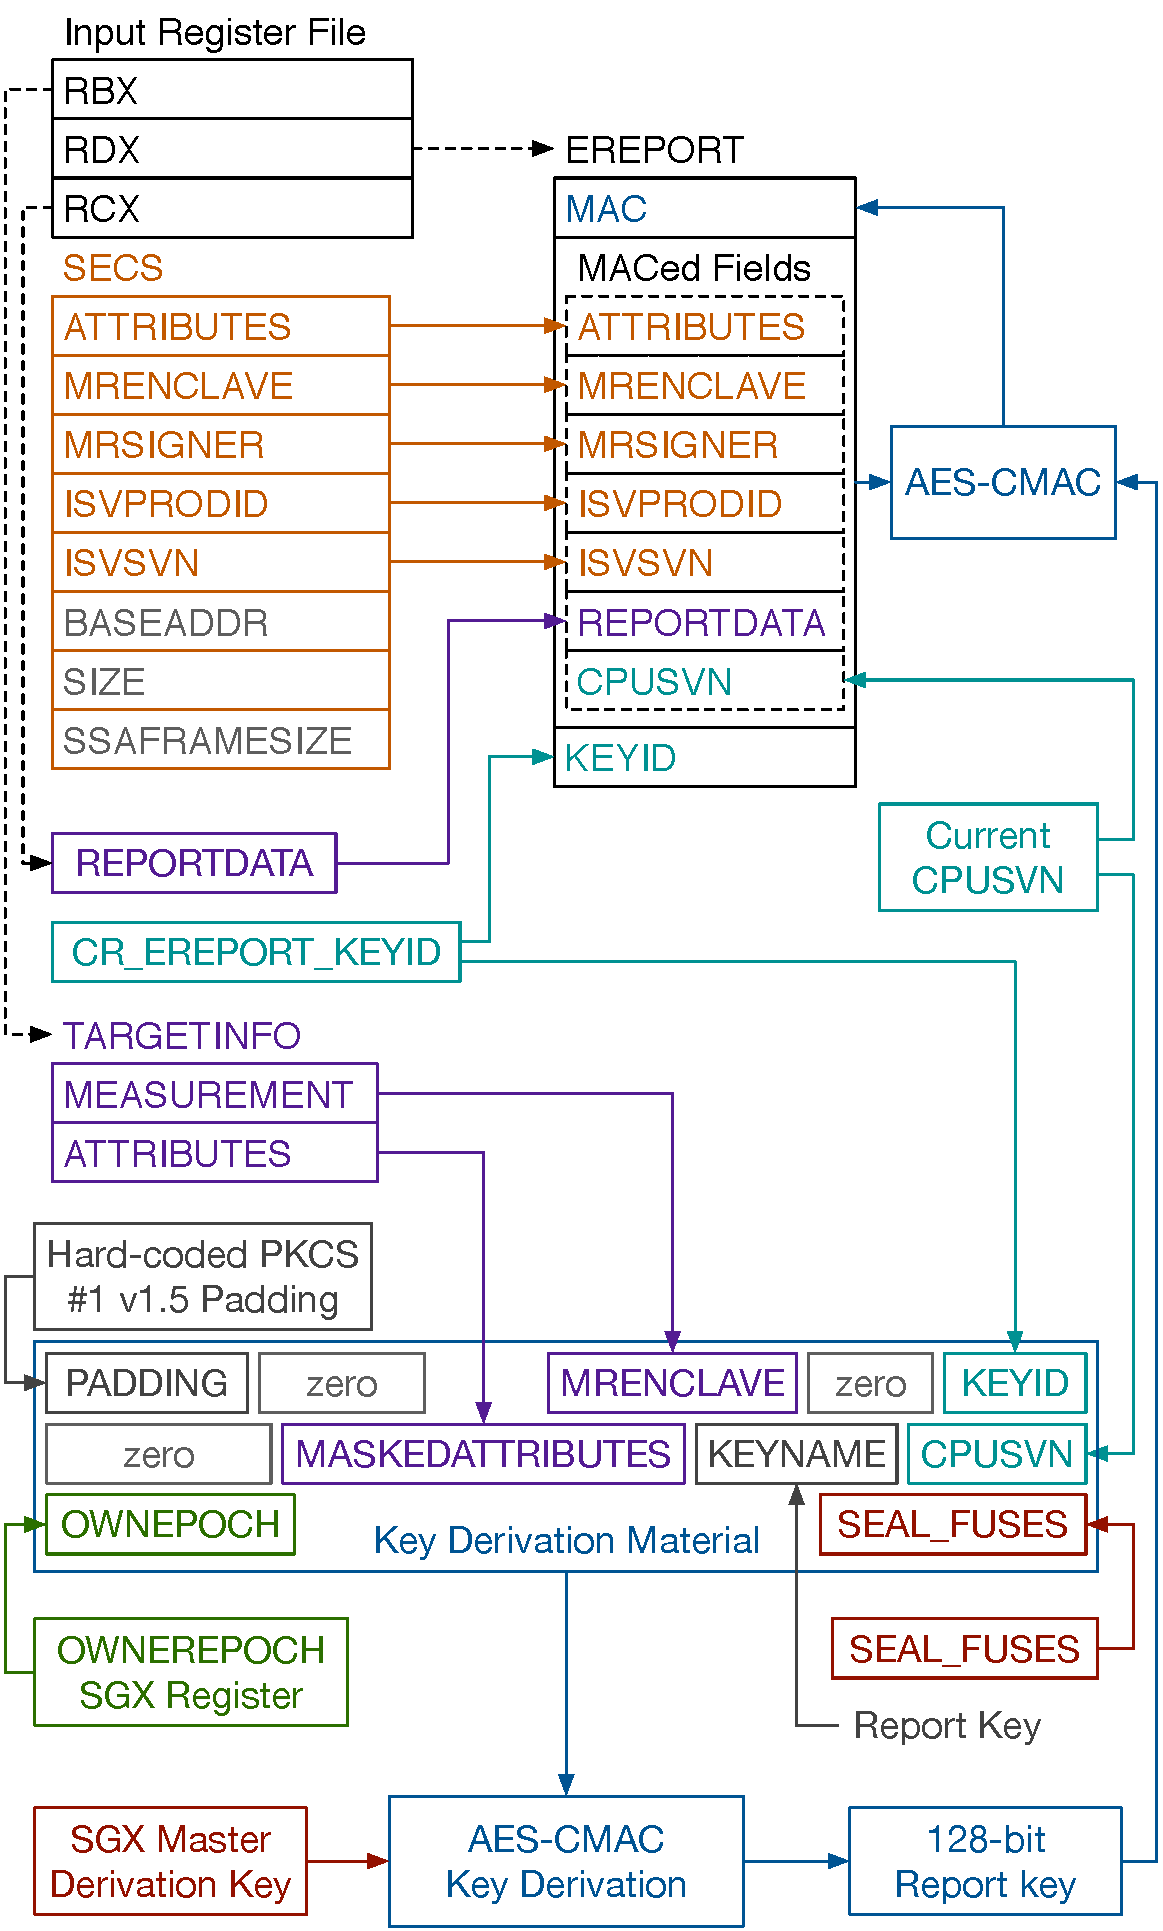
\includegraphics[width=85mm]{figures/sgx_ereport.pdf}
  \caption{
    \texttt{EREPORT} data flow
  }
  \label{fig:sgx_ereport}
\end{figure}

The \texttt{EREPORT} instruction reads the current enclave's identity
information from the enclave's SECS~(\S~\ref{sec:sgx_secs}), and uses it to
populate the REPORT structure. Specifically, \texttt{EREPORT} copies the
SECS fields indicating the enclave's measurement (MRENCLAVE), certificate-based
identity (MRSIGNER, ISVPRODID, ISVSVN), and attributes (ATTRIBUTES). The
attestation report also includes the SVN of the SGX implementation (CPUSVN)
and a 64-byte (512-bit) message supplied by the enclave.

% Keys: SDM S 39.4.3

The target enclave that receives the attestation report can convince itself of
the report's authenticity as shown in Figure~\ref{fig:sgx_ereport_check}. The
report's authenticity proof is its MAC tag. The key required to verify the MAC
can only be obtained by the target enclave, by asking
\texttt{EGETKEY}~(\S~\ref{sec:sgx_egetkey}) to derive a Report key. The SDM
states that the MAC tag is computed using a block cipher-based
MAC~(CMAC,~\cite{fips2005cmac}), but stops short of specifying the underlying
cipher. One of the SGX papers~\cite{anati2013sgx} states that the CMAC is based
on 128-bit AES.

\begin{figure}[hbt!]
  \centering
  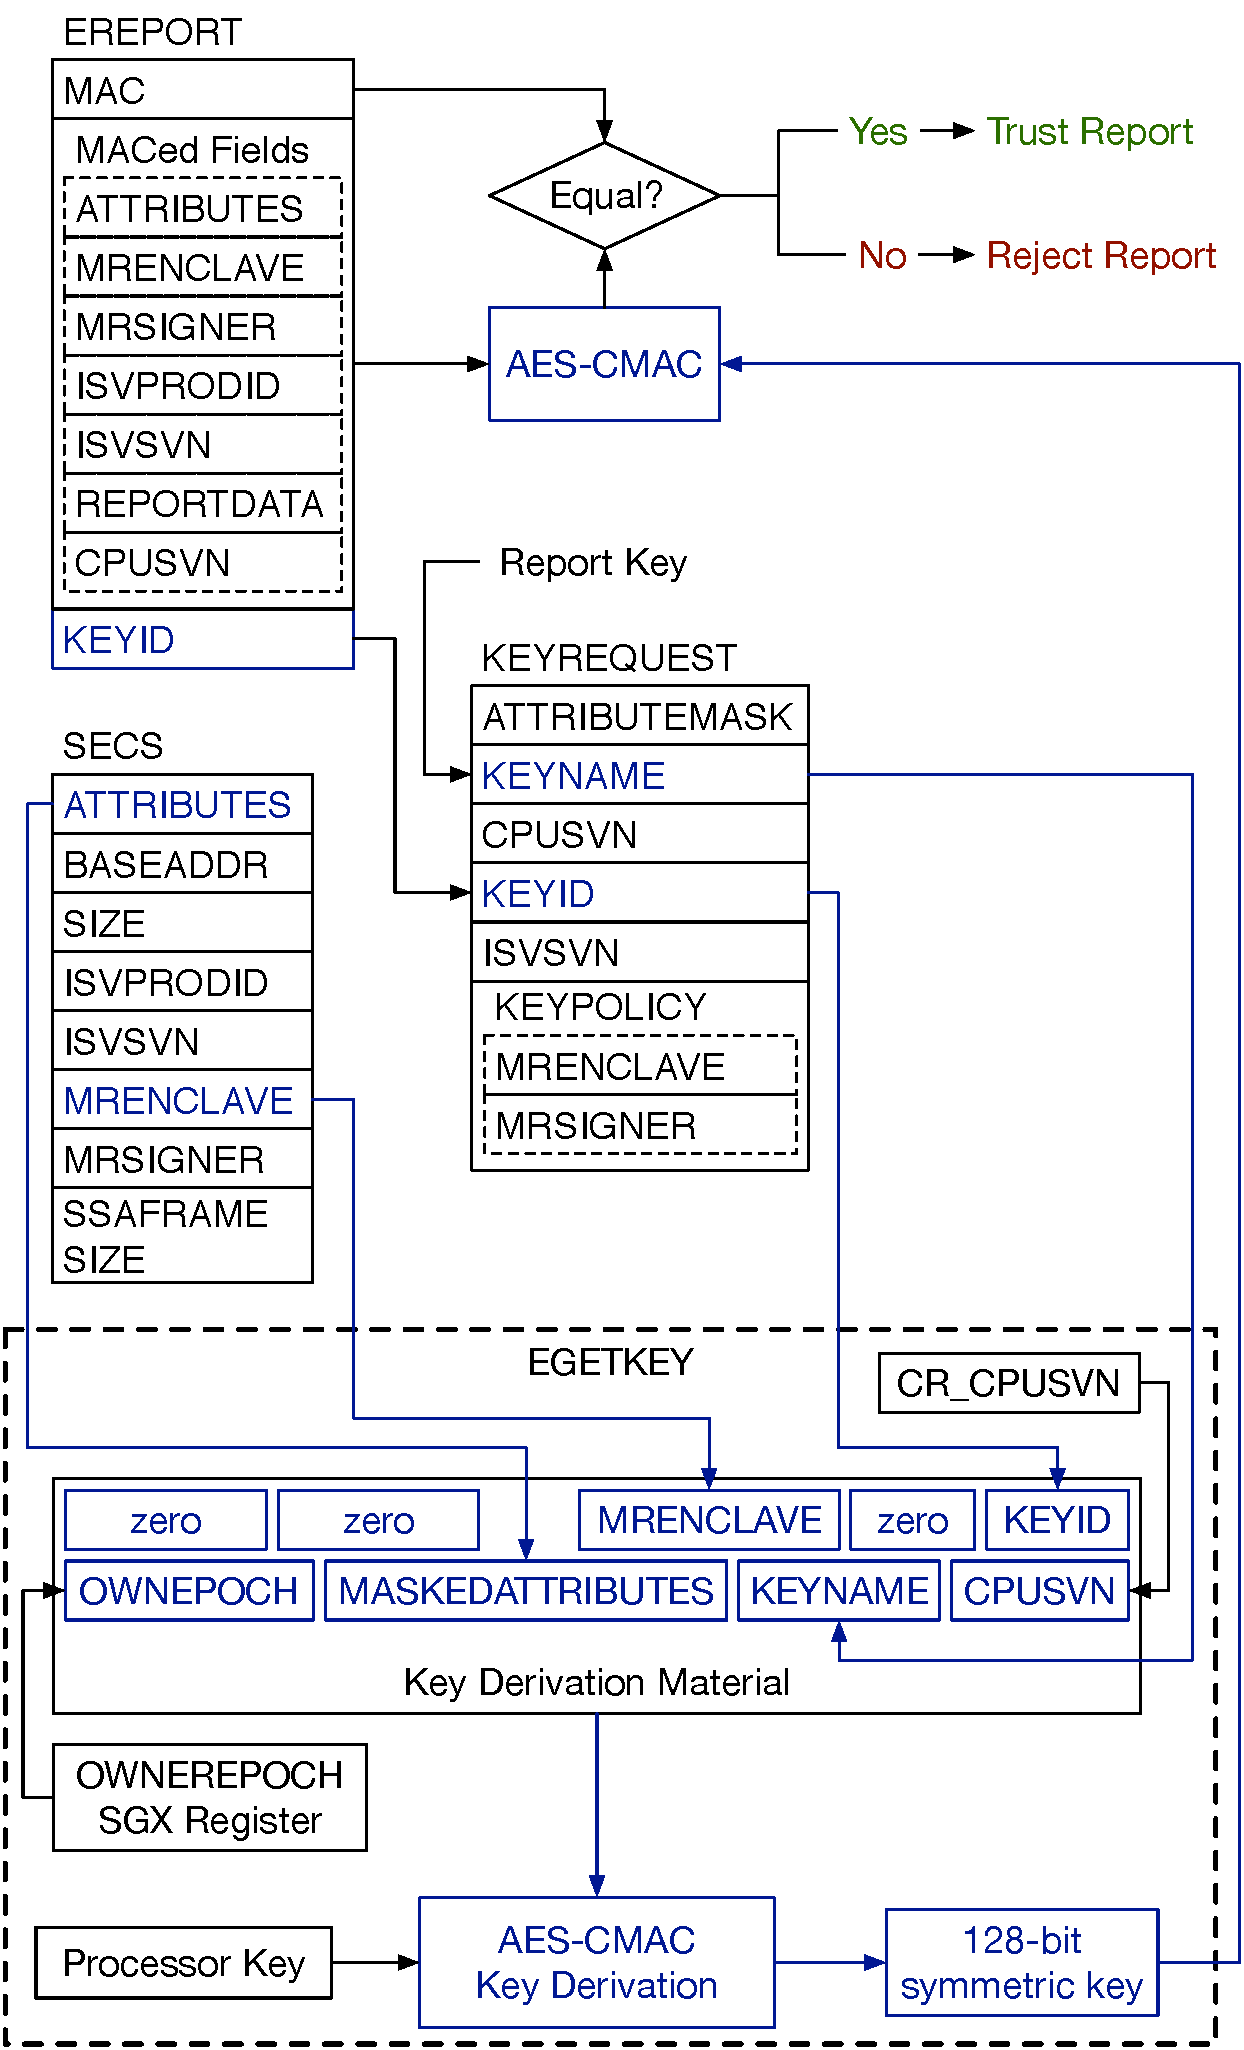
\includegraphics[width=87mm]{figures/sgx_ereport_check.pdf}
  \caption{
    The authenticity of the REPORT structure created by \texttt{EREPORT} can
    and should be verified by the report's target enclave. The target's code
    uses \texttt{EGETKEY} to obtain the key used for the MAC tag embedded in
    the REPORT structure, and then verifies the tag.
  }
  \label{fig:sgx_ereport_check}
\end{figure}

The Report key returned by \texttt{EGETKEY} is derived from a secret embedded
in the processor~(\S~\ref{sec:sgx_egetkey}), and the key material includes the
target enclave's measurement. The target enclave can be assured that the MAC
tag in the report was produced by the SGX implementation, for the following
reasons. The cryptographic properties of the underlying key derivation and
MAC algorithms ensure that only the SGX implementation can produce the MAC tag,
as it is the only entity that can access the processor's secret, and it would
be impossible for an attacker to derive the Report key without knowing the
processor's secret. The SGX design guarantees that the key produced by
\texttt{EGETKEY} depends on the calling enclave's measurement, so only the
target enclave can obtain the key used to produce the MAC tag in the report.

\texttt{EREPORT} uses the same key derivation process as \texttt{EGETKEY}
does when invoked with KEYNAME set to the value associated with Report keys.
For this reason, \texttt{EREPORT} requires the virtual address of a
\textit{Report Target Info}~(TARGETINFO) structure that contains the
measurement-based identity and attributes of the target enclave.

% EGETKEY: SDM S 41.4.1
% Key Derivation: SDM Table 41-43

When deriving a Report key, \texttt{EGETKEY} behaves slightly differently than
it does in the case of seal keys, as shown in
Figure~\ref{fig:sgx_ereport_check}. The key generation material never includes
the fields corresponding to the enclave's certificate-based identity (MRSIGNER,
ISVPRODID, ISVSVN), and the KEYPOLICY field in the KEYREQUEST structure is
ignored. It follows that the report can only be verified by the target enclave.

Furthermore, the SGX implementation's SVN~(CPUSVN) value used for key generation
is determined by the current CPUSVN, instead of being read from the Key Request
structure. Therefore, SGX implementation upgrades that increase the CPUSVN
invalidate all outstanding reports. Given that CPUSVN increases are associated
with security fixes, the argument in \S~\ref{sec:sgx_certificate_identity}
suggests that this restriction may reduce the impact of vulnerabilities in the
SGX implementation.

Last, \texttt{EREPORT} sets the KEYID field in the key generation material to
the contents of an SGX configuration register (CR\_REPORT\_KEYID) that is
initialized with a random value when SGX is initialized. The KEYID value is
also saved in the attestation report, but it is not covered by the MAC tag.

% EREPORT key derivation
%   US 8,972,746 B2 - 21:51-67, 22:1-6, Figure 12
% EREPORT uses KeyID which is incremented after 2^32 AES operations
%   US 8,972,746 B2 - 22:7-12
% EREPORT's MAC is actually a GMAC, not a CMAC
%   US 8,972,746 B2 - 21:64-67


\HeadingLevelC{Remote Attestation}
\label{sec:sgx_quoting_enclave}

The SDM paints a complete picture of the local attestation mechanism that was
described in \S~\ref{sec:sgx_ereport}. The remote attestation process, which
includes the Quoting Enclave and the underlying keys, is covered at a high
level in an Intel publication~\cite{johnson2016sgxprovisioning}. This section's
contents is based on the SDM, on one~\cite{anati2013sgx} of the SGX papers, and
on the ISCA 2015 SGX tutorial~\cite{intel2015iscasgx}.

% Keys: SDM S 39.4.3
% ISCA 2015 SGX Slides 104, 105, 106
% ISCA 2015 SGX Slide 105:
%   "Intel generates and fuses a unique key during manufacturing"
%   "Intel maintains a database of these keys."
% ISCA 2015 SGX Slide 235:
%   "Security Service" bubble includes "Launching", "Quoting", "Provisioning"

SGX's software attestation scheme, which is illustrated in
Figure~\ref{fig:sgx_attestation_keys}, relies on a key generation facility and
on a provisioning service, both operated by Intel.

\begin{figure}[hbt]
  \centering
  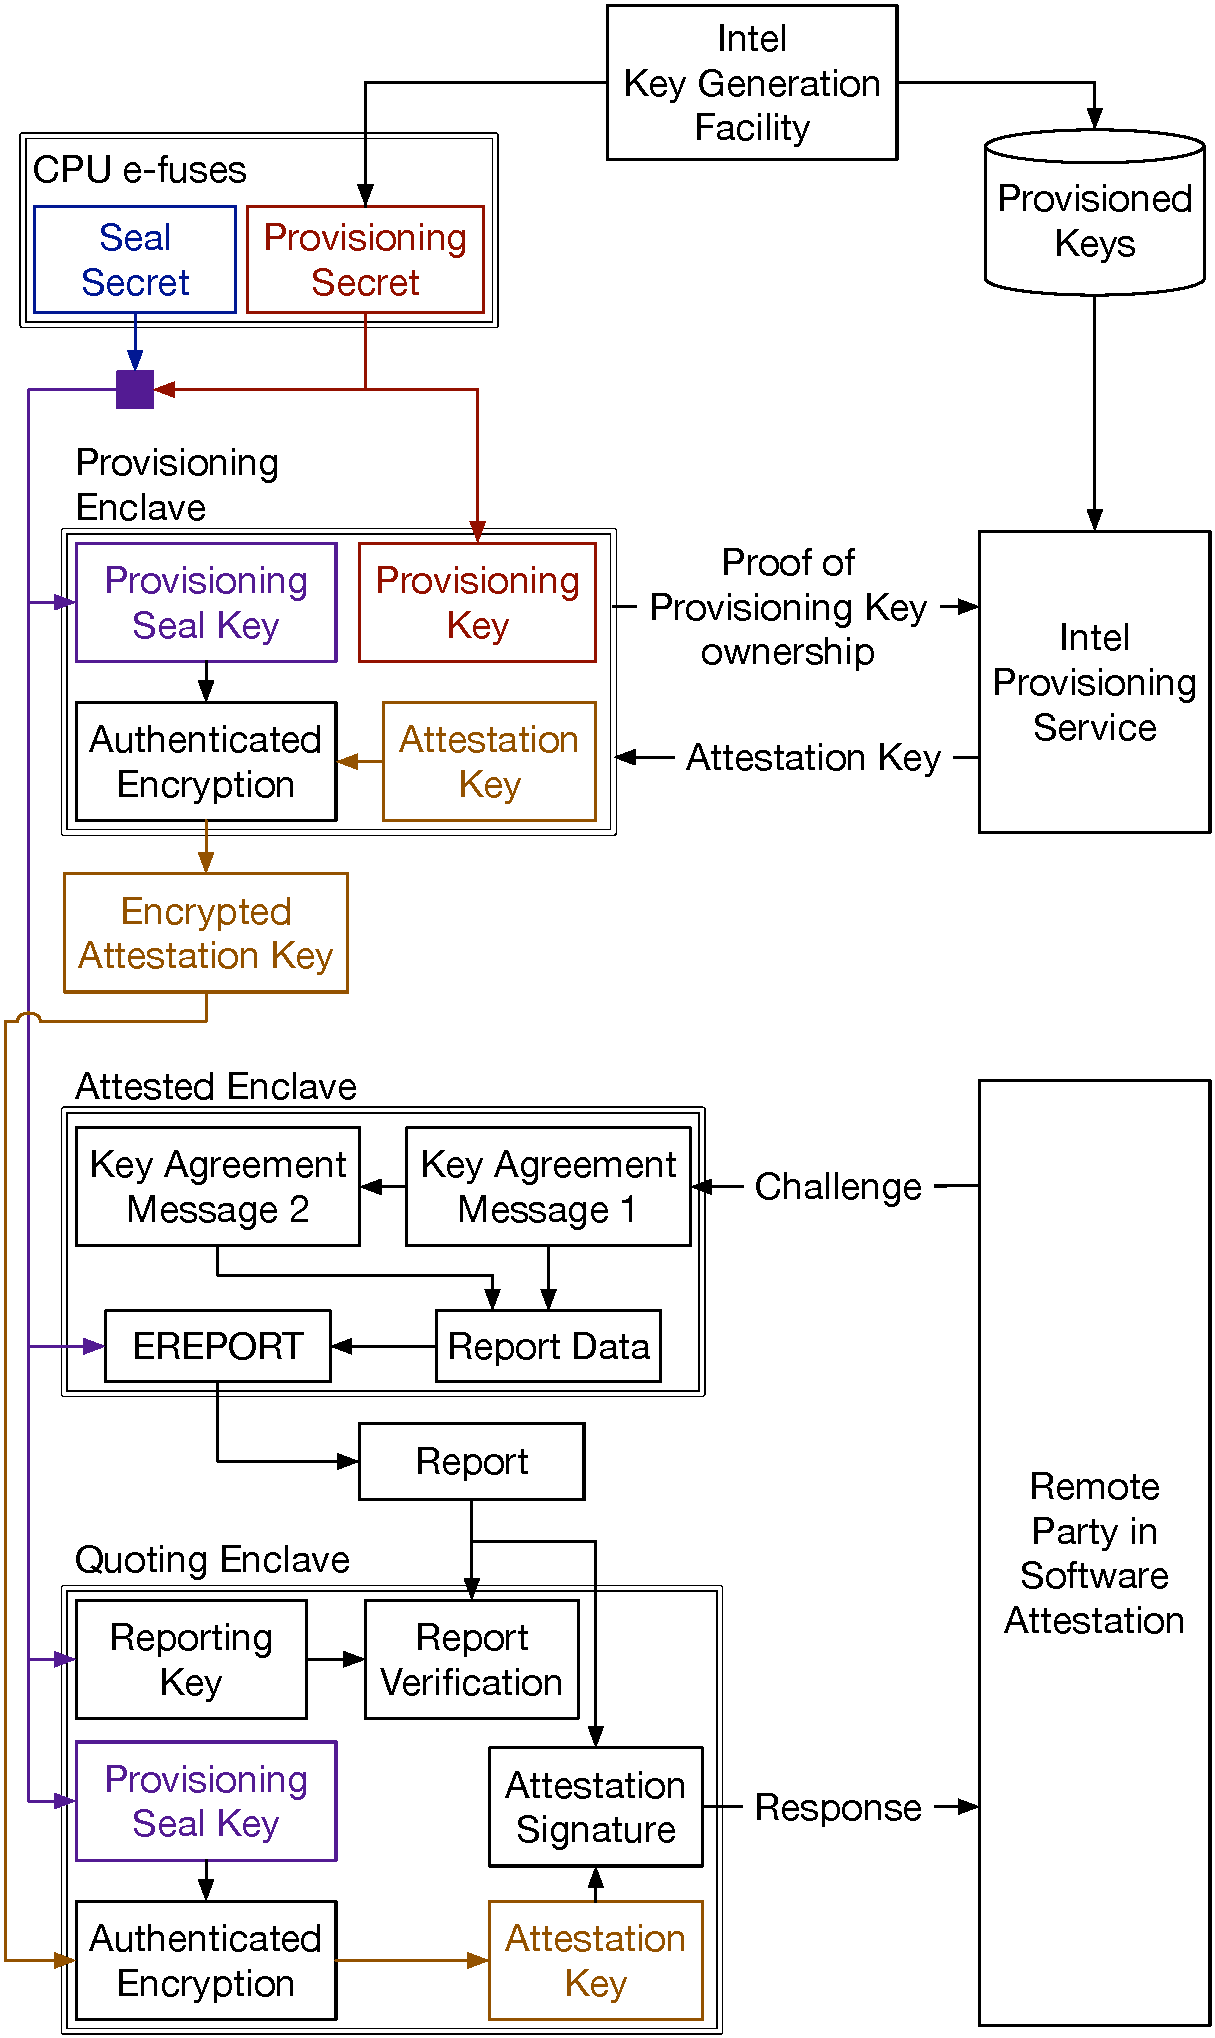
\includegraphics[width=85mm]{figures/sgx_attestation_keys.pdf}
  \caption{
    SGX's software attestation is based on two secrets stored in e-fuses inside
    the processor's die, and on a key received from Intel's provisioning
    service.
  }
  \label{fig:sgx_attestation_keys}
\end{figure}

During the manufacturing process, an SGX-enabled processor communicates with
Intel's key generation facility, and has two secrets burned into e-fuses, which
are a one-time programmable storage medium that can be economically included on
a high-performance chip's die. We shall refer to the secrets stored in e-fuses
as the \textit{Provisioning Secret} and the \textit{Seal Secret}.

% EGETKEY: SDM S 41.4.1
% Key Derivation: SDM Table 41-43

The Provisioning Secret is the main input to a largely undocumented process
that outputs the SGX master derivation key used by \texttt{EGETKEY}, which was
referenced in Figures \ref{fig:sgx_egetkey},
\ref{fig:sgx_attestation_overview}, \ref{fig:sgx_ereport}, and
\ref{fig:sgx_ereport_check}.
%
% TODO(pwnall): Uncomment the sentence below when/if we have the new keys
%               section ready.
%
% \S~\ref{sec:sgx_hardware_keys} will attempt to
% shed light on this undocumented process by fusing the information from the
% ISCA 2015 SGX tutorial with the SGX patents.

The Seal Secret is not exposed to software by any of the architectural
mechanisms documented in the SDM. The secret is only accessed when it is
included in the material used by the key derivation process implemented by
\texttt{EGETKEY}~(\S~\ref{sec:sgx_egetkey}). The pseudocode in the SDM uses the
CR\_SEAL\_FUSES register name to refer to the Seal Secret.

The names ``Seal Secret'' and ``Provisioning Secret'' deviate from Intel's
official documents, which confusingly use the ``Seal Key'' and ``Provisioning
Key'' names to refer to both secrets stored in e-fuses and keys derived by
\texttt{EGETKEY}.

The SDM briefly describes the keys produced by \texttt{EGETKEY}, but no
official documentation explicitly describes the secrets in e-fuses. The
description below is is the only interpretation of all the public information
sources that is consistent with all the SDM's statements about key derivation.

The Provisioning Secret is generated at the key generation facility, where it
is burned into the processor's e-fuses and stored in the database used by
Intel's provisioning service. The Seal Secret is generated inside the processor
chip, and therefore is not known to Intel. This approach has the benefit that
an attacker who compromises Intel's facilities cannot derive most keys produced
by \texttt{EGETKEY}, even if the attacker also compromises a victim's firmware
and obtains the OWNEREPOCH~(\S~\ref{sec:sgx_egetkey}) value. These keys include
the Seal keys~(\S~\ref{sec:sgx_egetkey}) and Report
keys~(\S~\ref{sec:sgx_ereport}) introduced in previous sections.

The only documented exception to the reasoning above is the
\textit{Provisioning key}, which is effectively a shared secret between the
SGX-enabled processor and Intel's provisioning service. Intel has to be able to
derive this key, so the derivation material does not include the Seal Secret or
the OWNEREPOCH value, as shown in Figure~\ref{fig:sgx_egetkey_provision}.

\begin{figure}[hbt]
  \centering
  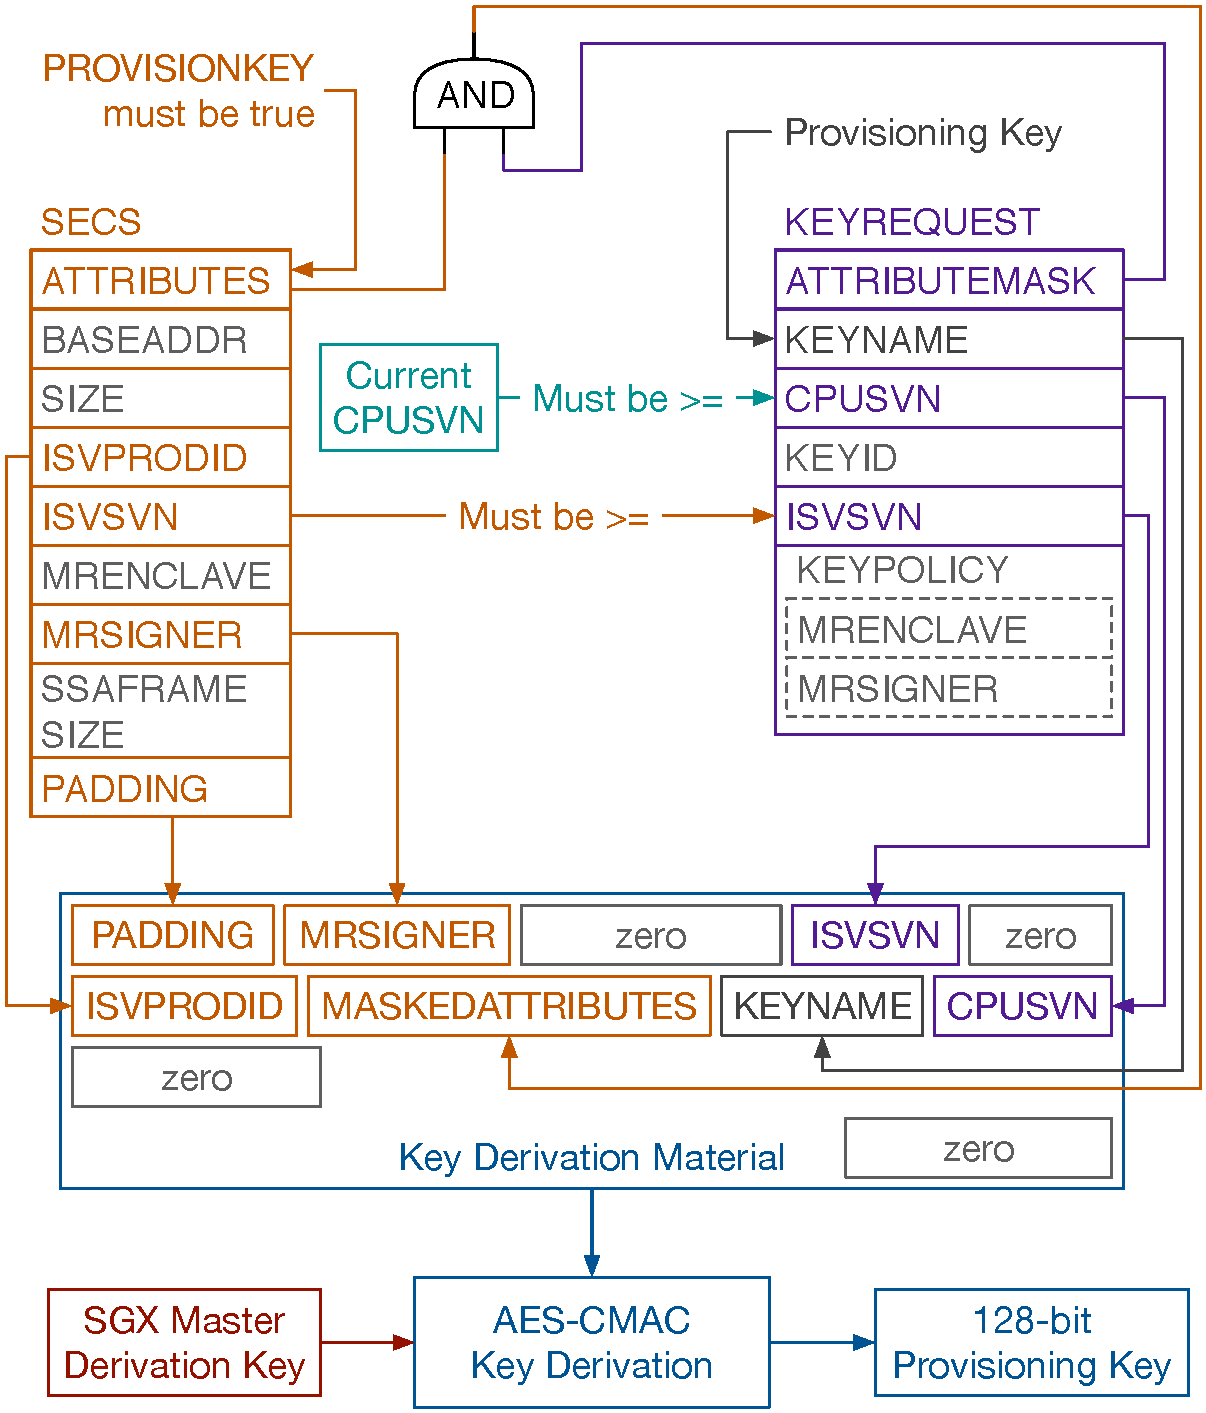
\includegraphics[width=87mm]{figures/sgx_egetkey_provision.pdf}
  \caption{
    When \texttt{EGETKEY} is asked to derive a Provisioning key, it does not
    use the Seal Secret or OWNEREPOCH. The Provisioning key does, however,
    depend on MRSIGNER and on the SVN of the SGX implementation.
  }
  \label{fig:sgx_egetkey_provision}
\end{figure}

\texttt{EGETKEY} derives the Provisioning key using the current enclave's
certificate-based identity (MRSIGNER, ISVPRODID, ISVSVN) and the SGX
implementation's SVN (CPUSVN). This approach has a few desirable security
properties. First, Intel's provisioning service can be assured that it is
authenticating a Provisioning Enclave signed by Intel. Second, the provisioning
service can use the CPUSVN value to reject SGX implementations with known
security vulnerabilities. Third, this design admits multiple mutually
distrusting provisioning services.

\texttt{EGETKEY} only derives Provisioning keys for enclaves whose PROVISIONKEY
attribute is set to true. \S~\ref{sec:sgx_provisioning_privacy} argues
that this mechanism is sufficient to protect the computer owner from a
malicious software provider that attempts to use Provisioning keys to track a
CPU chip across OWNEREPOCH changes.

After the Provisioning Enclave obtains a Provisioning key, it uses the key to
authenticate itself to Intel's provisioning service. Once the provisioning
service is convinced that it is communicating to a trusted Provisioning enclave
in the secure environment provided by a SGX-enabled processor, the service
generates an \textit{Attestation Key} and sends it to the Provisioning Enclave.
The enclave then encrypts the Attestation Key using a
\textit{Provisioning Seal key}, and hands off the encrypted key to the system
software for storage.

Provisioning Seal keys, are the last publicly documented type of special keys
derived by \texttt{EGETKEY}, using the process illustrated in
Figure~\ref{fig:sgx_egetkey_provseal}. As their name suggests, Provisioning
Seal keys are conceptually similar to the Seal Keys~(\S~\ref{sec:sgx_egetkey})
used to migrate secrets between enclaves.

\begin{figure}[hbt]
  \centering
  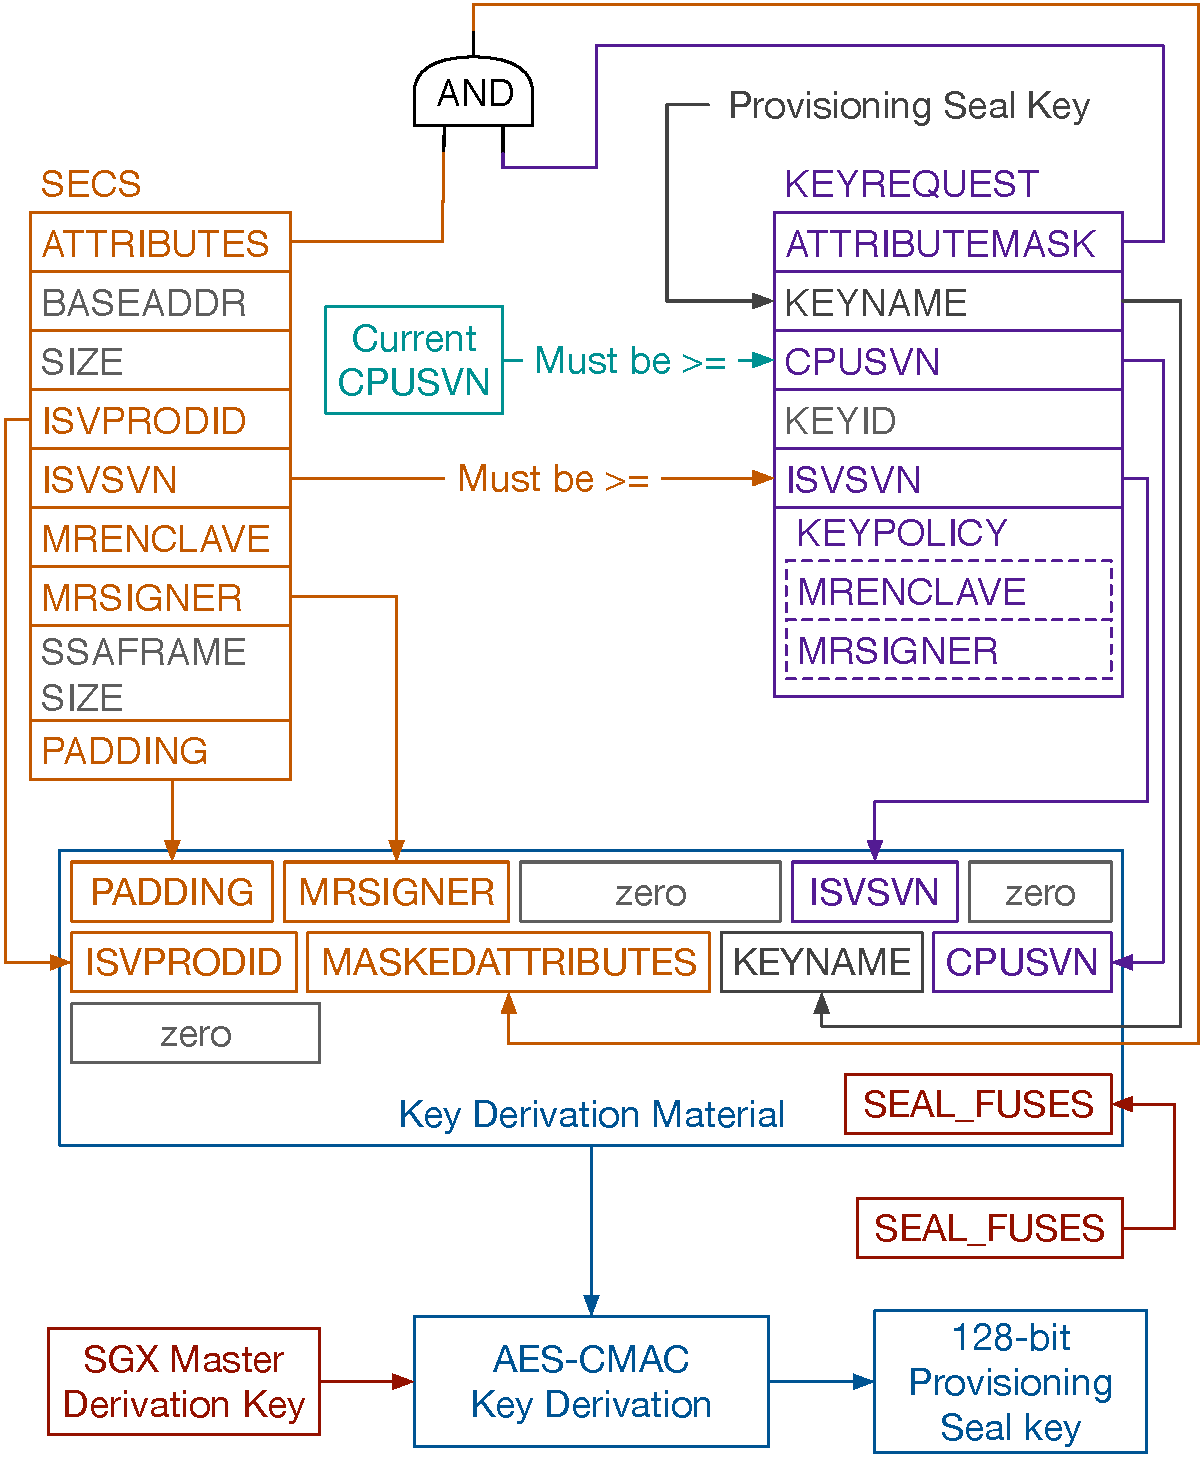
\includegraphics[width=87mm]{figures/sgx_egetkey_provseal.pdf}
  \caption{
    The derivation material used to produce Provisioning Seal keys does not
    include the OWNEREPOCH value, so the keys survive computer ownership
    changes.
  }
  \label{fig:sgx_egetkey_provseal}
\end{figure}

The defining feature of Provisioning Seal keys is that they are not based on
the OWNEREPOCH value, so they survive computer ownership changes. Since
Provisioning Seal keys can be used to track a CPU chip, their use is gated on
the PROVISIONKEY attribute, which has the same semantics as for Provisioning
keys.

Like Provisioning keys, Seal keys are based on the current enclave's
certificate-based identity (MRSIGNER, ISVPROD, ISVSVN), so the Attestation Key
encrypted by Intel's Provisioning Enclave can only be decrypted by another
enclave signed with the same Intel RSA key. However, unlike Provisioning keys,
the Provisioning Seal keys are based on the Seal Secret in the processor's
e-fuses, so they cannot be derived by Intel.

When considered independently from the rest of the SGX design, Provisioning
Seal keys have desirable security properties. The main benefit of these keys is
that when a computer with an SGX-enabled processor exchanges owners, it does
not need to undergo the provisioning process again, so Intel does not need to
be aware of the ownership change. The confidentiality issue that stems from not
using OWNEREPOCH was already introduced by Provisioning keys, and is mitigated
using the access control scheme based on the PROVISIONKEY attribute that will
be discussed in \S~\ref{sec:sgx_provisioning_privacy}.

Similarly to the Seal key derivation process, both the Provisioning and
Provisioning Seal keys depend on the bitwise AND of the
ATTRIBUTES~(\S~\ref{sec:sgx_secs_attributes}) field in the enclave's SECS and
the ATTRIBUTESMASK field in the KEYREQUEST structure. While most attributes can
be masked away, the DEBUG and INIT attributes are always used for key
derivation.

This dependency makes it safe for Intel to use its production RSA key to issue
certificates for Provisioning or Quoting Enclaves with debugging features
enabled. Without the forced dependency on the DEBUG attribute, using the
production Intel signing key on a single debug Provisioning or Quoting Enclave
could invalidate SGX's security guarantees on all the CPU chips whose
attestation-related enclaves are signed by the same key.
Concretely, if the issued SIGSTRUCT would be leaked, any attacker could build a
debugging Provisioning or Quoting enclave, use the SGX debugging features to
modify the code inside it, and extract the 128-bit Provisioning key used to
authenticated the CPU to Intel's provisioning service.

% Quoting Enclave replaces MAC in REPORT with attestation signature
%   HASP 2013 Attestation/Sealing paper, S 3.2

After the provisioning steps above have been completed, the Quoting Enclave can
be invoked to perform SGX's software attestation. This enclave receives local
attestation reports~(\S~\ref{sec:sgx_ereport}) and verifies them using the
Report keys generated by \texttt{EGETKEY}. The Quoting Enclave then obtains the
Provisioning Seal Key from \texttt{EGETKEY} and uses it to decrypt the
Attestation Key, which is received from system software. Last, the enclave
replaces the MAC in the local attestation report with an \textit{Attestation
Signature} produced with the Attestation Key.

% Quoting Enclave is a reference to the TPM
%   US 8,972,746 B2 - 20:59-67

The SGX patents state that the name ``Quoting Enclave'' was chosen as a
reference to the TPM~(\S~\ref{sec:sgx_related_tpm})'s quoting feature, which is
used to perform software attestation on a TPM-based system.

% ISCA 2015 SGX: Slides 105, 106

The Attestation Key uses Intel's \textit{Enhanced Privacy ID}~(EPID)
cryptosystem~\cite{brickell2009epid}, which is a group signature scheme that is
intended to preserve the anonymity of the signers. Intel's key provisioning
service is the issuer in the EPID scheme, so it publishes the Group Public Key,
while securely storing the Master Issuing Key. After a Provisioning Enclave
authenticates itself to the provisioning service, it generates an EPID Member
Private Key, which serves as the Attestation Key, and executes the EPID Join
protocol to join the group. Later, the Quoting Enclave uses the EPID Member
Private Key to produce Attestation Signatures.

The Provisioning Secret stored in the e-fuses of each SGX-enabled processor can
be used by Intel to trace individual chips when a Provisioning Enclave
authenticates itself to the provisioning service. However, if the EPID Join
protocol is blinded, Intel's provisioning service cannot trace an Attestation
Signature to a specific Attestation Key, so Intel cannot trace Attestation
Signatures to individual chips.

Of course, the security properties of the description above hinge on the
correctness of the proofs behind the EPID scheme. Analyzing the correctness of
such cryptographic schemes is beyond the scope of this work, so we defer the
analysis of EPID to the crypto research community.
